\documentclass[conference]{IEEEtran}
\IEEEoverridecommandlockouts
% The preceding line is only needed to identify funding in the first footnote. If that is unneeded, please comment it out.
\usepackage{cite}
\usepackage{amsmath,amssymb,amsfonts}
\usepackage{algorithmic}
\usepackage{graphicx}
\usepackage{textcomp}
\usepackage{xcolor}
\def\BibTeX{{\rm B\kern-.05em{\sc i\kern-.025em b}\kern-.08em
    T\kern-.1667em\lower.7ex\hbox{E}\kern-.125emX}}
\begin{document}

\title{Localization with activity recognition and particle filter\\}

\author{
\IEEEauthorblockN{1\textsuperscript{st} Bergauer Philipp}
\IEEEauthorblockA{\textit{TU Graz} \\
Graz, Austria\\
philipp.bergauer@student.tugraz.at
}
\and
\IEEEauthorblockN{2\textsuperscript{nd} Halici {\"O}mer Faruk}
\IEEEauthorblockA{\textit{TU Graz} \\
Graz, Austria\\
halici@student.tugraz.at}
}

\maketitle

\begin{abstract}
This document is a model and instructions for \LaTeX.
This and the IEEEtran.cls file define the components of your paper [title, text, heads, etc.]. *CRITICAL: Do Not Use Symbols, Special Characters, Footnotes, 
or Math in Paper Title or Abstract.
\end{abstract}

\begin{IEEEkeywords}
component, formatting, style, styling, insert
\end{IEEEkeywords}

\section{Introduction}
The Localization was splited into two parts, the first part was an Activity recognition and the second part was the localization Algorithm with the Particle Filter. The Activity recognition was implemented with an k-Nearest Neighbor(k-NN) algorithm. It was used to classify if the user is moving or not. 

\section{Activity recognition}
The mobile phone has many sensors. Some of them can be used to track the activity of a person.  After collecting sensor data the patterns in the data can be retrieved and can be used to classify between activities e.g jogging,running, walking.
\subsection{Tensorflow approach for Convolutional Neural Network}
Our first approach was to use the popular tensorflow framework from Google. The idea was to train and write the cody in python and export a tensorflow model which can be used by our mobile phone. The trainingsdata was taken from the Wireless Sensor Data Mining group\cite{b1}. We decided to use a CNN network because it can be used to analyze interesting fatures in the data set. The error rate for the trainings data was very low. Only 15 \% were missclassified. The export to the android device worked too but in the end it did not work as accurate enough. The problem was that our dataset and our own sensor data generated from our mobile phones were to different so the model missclassified most of the activites wrong. Afterwards we tried to After days of debugging and fixing errors we came to the conclusion to go along with the K-NN approach\cite{b2}.
\subsection{K-NN approach}
First of all the K-NN algorithm is one of the simplest and most used classification algorithms. The classification of an object/class uses the majority vote of its neighbours. There are many decisions to be made before implementing the K-NN. First of all which K should we take. The K stands for the number of neighbours to be taken in account. It should be an odd number. In our case it was 21. The calculation of the distance is another point to think about. We decided to use the euclidean distance for our K-NN. The formula of the euclidean distance:
\begin{equation}
D(w_i,v_i) = \sqrt{\sum{(w_i - v_i)^2}}
\end{equation}
The euclidean distance is easy to program and is very efficient. 
\subsection{Feature extraction}
Afterwards we thought about the features to use for the data set and the window size. We took the same features as for our CNN.The mean for each axis of the accelerometer values, the max peaks in each axis,the min peaks in each axis and the variances of each axis. 
In addition one record contains 20 samples too. The sample rate can be adjusted in android so we took the sampling rate $SENSOR\_DELAY\_FASTEST$. According to its name it should be the fastest one. The windows size are 20 samples. The sampling rate is dependable on the hardware in the mobile phone, so it is hard to give a window for 20 samples in seconds but it should be approximately 50ms. 
\subsection{Data generation}
The reference dataset was  taken with the SensorHandler. These class takes the samples and writed them in a txt file. In our main activity we can click on the generate data button and generate data for our classificitation as shown in 
\ref{fig:mainmenuactivity}. \\ 
\begin{figure}
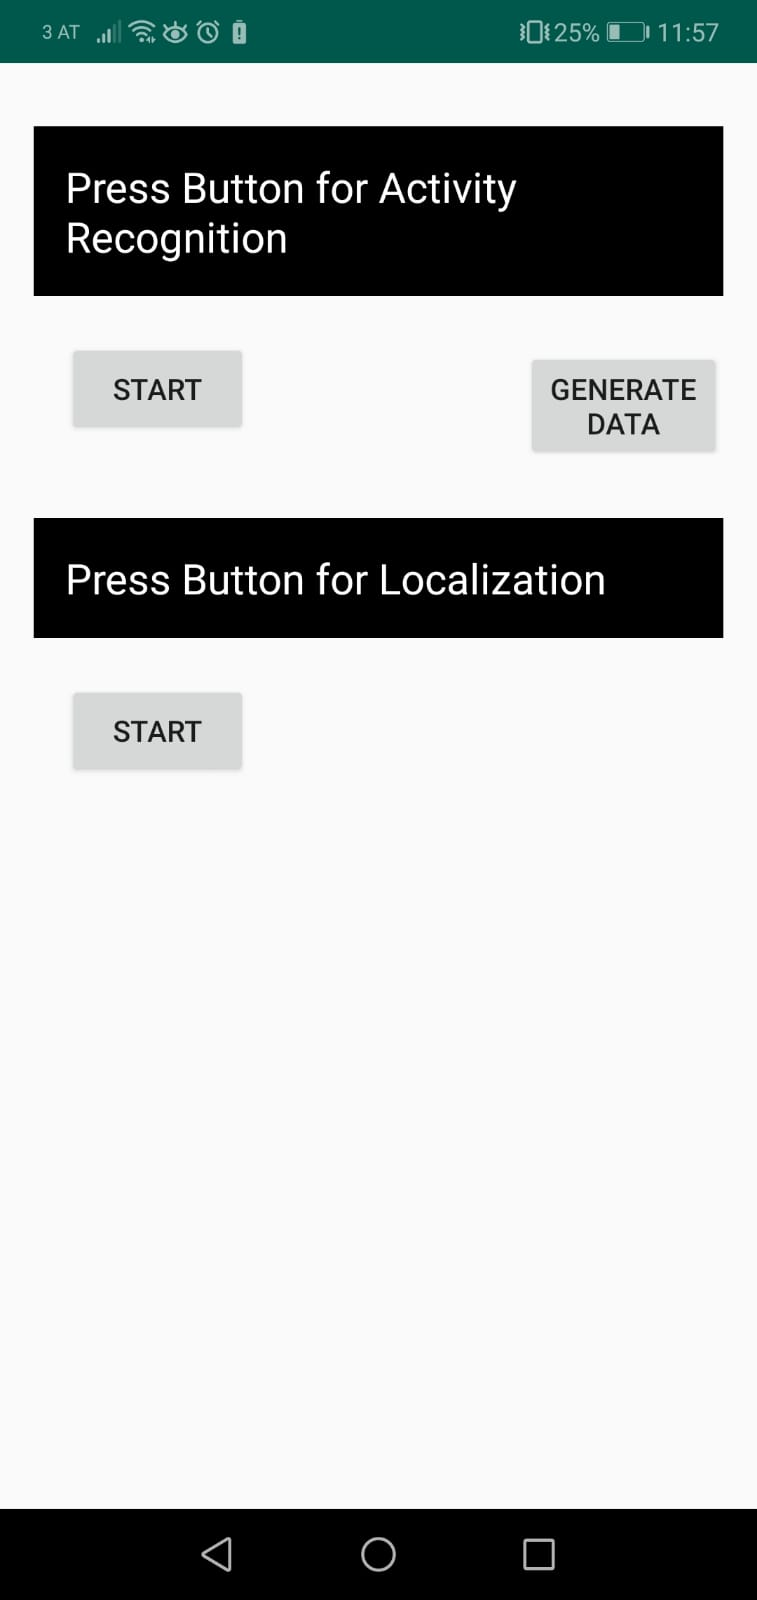
\includegraphics[height = 7.5cm,width = 5cm]{Images/MainActivity.jpeg}
\centering
\caption{MainMenuActivity of the application}
\label{fig:mainmenuactivity}
\end{figure}\\
With our own dataset and the extracted features we could classify. We differentiated between 3 classes:Walking,Standing and Sitting. It should be explicitly noted that our activity recognition works with the phone in the pocket. 
\subsection{Classifier}
\begin{figure}
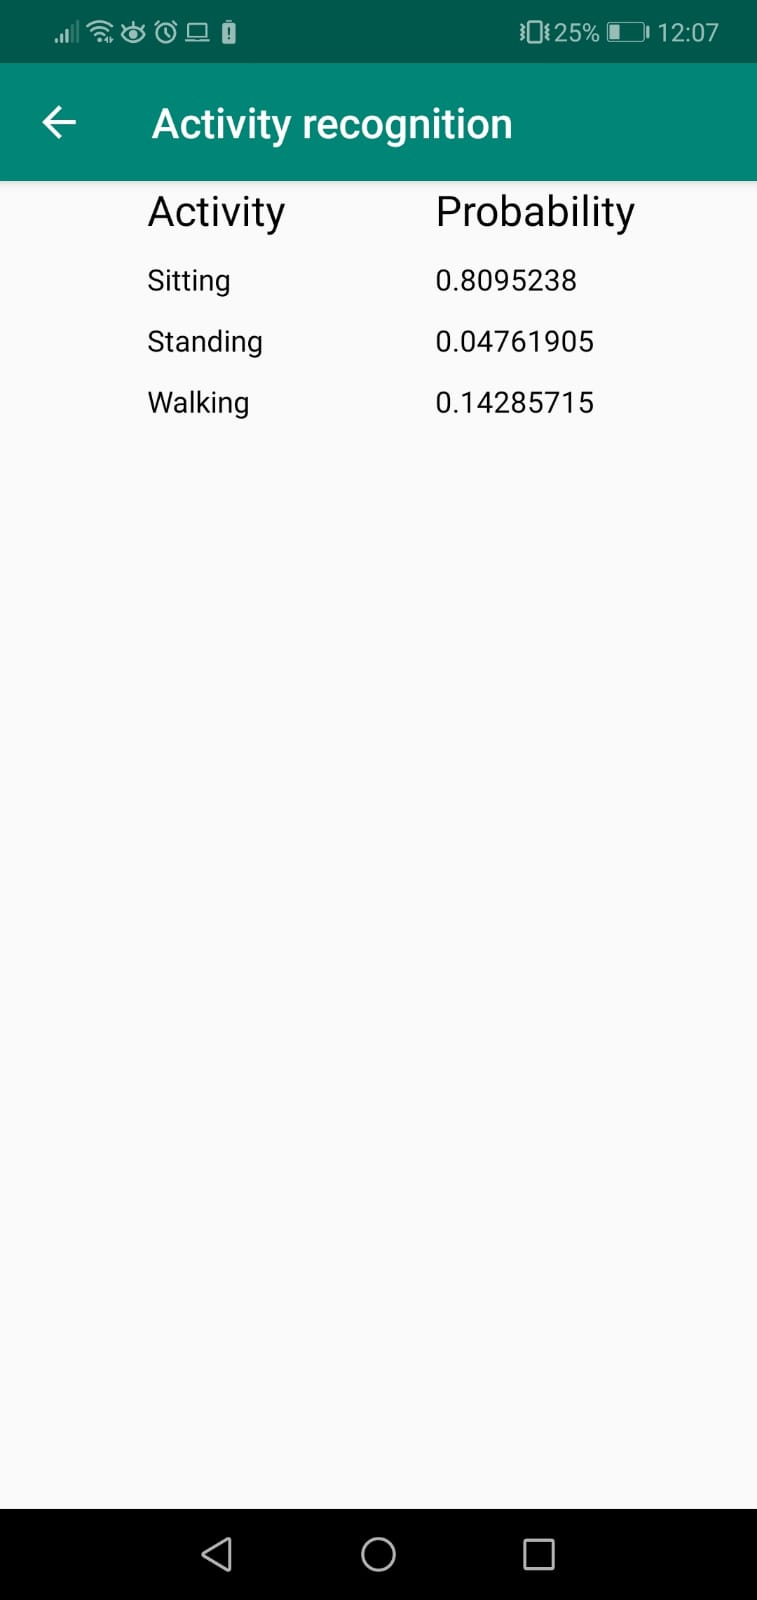
\includegraphics[height = 7.5cm,width = 5cm]{Images/AcitivityRecognition.jpeg}
\centering
\caption{Activityrecognition with accelerometer values }
\label{fig:classifier}
\end{figure}
As seen in \ref{fig:classifier} the K-NN algorithm classified sitting right with an accuracy about 80 \%. The classifier is very fast because we use the fastest sampling rate possible. The best classification are walking and standing because the accelerometer values are much apparent to our classifier.
Before you begin to format your paper, first write and save the content as a 
separate text file. Complete all content and organizational editing before 
formatting. Please note sections \ref{AA}--\ref{SCM} below for more information on 
proofreading, spelling and grammar.

Keep your text and graphic files separate until after the text has been 
formatted and styled. Do not number text heads---{\LaTeX} will do that 
for you.


\section*{Localization}

The preferred spelling of the word ``acknowledgment'' in America is without 
an ``e'' after the ``g''. Avoid the stilted expression ``one of us (R. B. 
G.) thanks $\ldots$''. Instead, try ``R. B. G. thanks$\ldots$''. Put sponsor 
acknowledgments in the unnumbered footnote on the first page.


\subsection*{Floorplan}
For the Paritcle Filter to Work, an Floorplan of the building were we want to classify the position of the user is needed. So an floorplan of the 16 Inffeldgasse building is taken and edited, All the sections that should not be classified are coloured light grey. Then because the wall has Pixel holes an wall finding Algorithm was written and the walls were colored red so continues walls were created. In the floor plan was a scale were one rectangle was 5 meters, so that was coloured green and then our programm looked how wide one rectangle was and calculated how many Pixels the rectangle was wide, so an factor for Meter to Pixel was created. After this the orientation sensor has to be calibrated for the building, to have the perfect angle we added an offset of 47 degress to our orientation. So with this method our programm can be used on every building with very little things to rethink.


\subsection*{Particle Filter}

After everything with the floorplan was done the Particle Filter was implemented. 
First the Particle Filter executes the init step. In the init step the Particle Filter distributes random 15000 Particle in the sections of the Floorplan that should be classified. All this Particles have a weight of $\frac{1}{15000} $ where the 15000 are the number of particles distributed.
Then when the Motion Model classifies that the user started moving the particles starts moving in the direction and distance the user is moving. For each Particle an bias is added to the movement direction and distance of the user so not all particles are moving the same. This is to work against uncertainness of the movement. When an Particle collides with an wall of the floorplan or is in an Position it's not allowed to be the weight of the particle is set to 0. All particles that are still valid are get a new weight. The weight is  $\frac{1}{num_particles_survived} $. After this step the Algorithm checks is a weight of a particle is 0 it is distributed new. The new Position of the invalid Particle is an Position of an old Particle. Because of the Bias that is added to the movment and orientation in the next step the Particles should be on different positions. The new resampled Particles get an weight of $\frac{1}{15000}.$. For the estimated Position the x and y Position for each Paritcle is taken and an median Filter is applied on the x and y postion. So the estimated position is the middle x and the middle y position of all Particles.


\subsection*{Optimizations particle filter}
\begin{thebibliography}{00}
\bibitem{b1} Jennifer R. Kwapisz, Gary M. Weiss, Samuel A. Moore, ``Activity Recognition using Cell Phone Accelerometers,''  Department of Computer and Information Science  Fordham University  441 East Fordham Road  Bronx, NY 10458.
\bibitem{b2}https://aqibsaeed.github.io/2016-11-04-human-activity-recognition-cnn/
\bibitem{b3} I. S. Jacobs and C. P. Bean, ``Fine particles, thin films and exchange anisotropy,'' in Magnetism, vol. III, G. T. Rado and H. Suhl, Eds. New York: Academic, 1963, pp. 271--350.
\bibitem{b4} K. Elissa, ``Title of paper if known,'' unpublished.
\bibitem{b5} R. Nicole, ``Title of paper with only first word capitalized,'' J. Name Stand. Abbrev., in press.
\bibitem{b6} Y. Yorozu, M. Hirano, K. Oka, and Y. Tagawa, ``Electron spectroscopy studies on magneto-optical media and plastic substrate interface,'' IEEE Transl. J. Magn. Japan, vol. 2, pp. 740--741, August 1987 [Digests 9th Annual Conf. Magnetics Japan, p. 301, 1982].
\bibitem{b7} M. Young, The Technical Writer's Handbook. Mill Valley, CA: University Science, 1989.
\end{thebibliography}
\vspace{12pt}
\color{red}
IEEE conference templates contain guidance text for composing and formatting conference papers. Please ensure that all template text is removed from your conference paper prior to submission to the conference. Failure to remove the template text from your paper may result in your paper not being published.

\end{document}
